\documentclass{article}
\usepackage{style-notes}

\newcounter{lecnum} 	% define counter for lecture number
\renewcommand{\thepage}{\thelecnum-\arabic{page}}	% define how page number is displayed (< lecture number > - < page number >)
% define lecture header and page numbers
% NOTE: to call use \lecture{< Lecture # >, < Lecture name >, < Chapter # >, < Chapter name >, < Section #s >}
\newcommand{\lecture}[5]{

    % define headers for first page
    \thispagestyle{empty} % removes page number from page where call is made

    \setcounter{lecnum}{#1}		% set lecture counter to argument specified

    % define header box
    \begin{center}
    \framebox{
      \vbox{\vspace{2mm}
    \hbox to 6.28in {\textbf{MATH 320: Probability} \hfill}
       \vspace{4mm}
       \hbox to 6.28in {{\hfill \Large{Lecture #1: #2} \hfill}}
       \vspace{2mm}
       \hbox to 6.28in {\hfill Chapter #3: #4 \small{(#5)}}
      \vspace{2mm}}
    }
    \end{center}
    \vspace{4mm}
    
    % define headers for subsequent pages
    \fancyhead[LE]{\textit{#2} \hfill \thepage} 		% set left header for even pages
    \fancyhead[RO]{\hfill \thepage}		% set right header for odd pages

}



% define macros (/shortcuts)
\newcommand{\bu}[1]{\textbf{\ul{#1}}}			% shortcut bold and underline text in one command
\newcommand{\blankul}[1]{\rule[-1.5mm]{#1}{0.15mm}}	% shortcut for blank underline, where the only option needed to specify is length (# and units (cm or mm, etc.)))
\newcommand{\vecn}[2]{#1_1, \ldots, #1_{#2}}		% define vector (without parentheses, so when writing out in like a definition) of the form X_1, ..., X_n, where X and n are variable. NOTE: to call use $\vecn{X}{n}$
\newcommand{\vecinf}[1]{#1_1, #1_{2}, \ldots}		% define another vector of the form X_1, X_2, ....
\newcommand{\comp}[1]{{\sim}#1}		% shortcut for complement of event ~A (tilde without extra space)

% NOTES on what didn't cover
% theory lecture 1 -> formal definitions of subset A subset B: if x in A => x in B
% same thing for all other definitions
% distributive law proof

\begin{document}

\lecture{1}{Set Theory}{1}{Probability}{1.1}

\bu{Where does data come from}\bigskip

Definitions\bigskip
\begin{itemize}
    \item An \textbf{experiment} is the process by which an observation/outcome is made, which cannot be predicted with certainty (outcomes are random).
    \item An \textbf{outcome} of an experiment is any possible observation of that experiment (often called sample points).
\end{itemize}\bigskip

Examples: Write the set of all possible outcomes for the following experiments.\bigskip
\begin{enumerate}
    \item Sampling students and computing the average number of study hours each day:\vspace{20pt}
    \item Roll die, record number that appears:\vspace{20pt}
    \item Roll die, record first role that a one appears:\vspace{20pt}
\end{enumerate}

\bu{What is probability and how to calculate it}\bigskip

Intuitively, probability is the likelihood of something occurring.\bigskip

One approach (simplest case)\bigskip
\begin{itemize}
    \item \textbf{Probability by counting equally likely outcomes}
    \[
    \text{Probability of an event} = \hspace{200pt}
    \]
     \begin{itemize}\bigskip
        \item Example: Flip a fair coin, $P(\text{Heads}) = $\\
    \end{itemize}
    \item Events are not always equally likely, so cannot determine probabilities by counting. But there is a simple way to estimate that probability.
\end{itemize}\bigskip\bigskip

Another approach\bigskip
\begin{itemize}
    \item \textbf{Empirical probability} (based on collected data).
    \item Relative frequency estimate of the probability of an event
    \[
    \text{Probability of an event} = \hspace{200pt}
    \]
    \item These are two ways of looking at probability.
    \begin{itemize}
        \item If outcomes are equally likely, \textit{relative frequency} $\approx$ \textit{counting} for a very large number of trials (e.g. if we simulated rolling a fair die 10,000 times, $\frac{\# \, 6s}{10,000} \approx \frac{1}{6}$).
        \begin{figure}[H]
            \center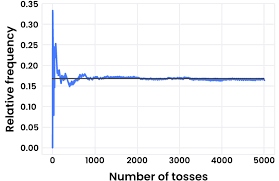
\includegraphics[scale=0.5]{test-1/rel-freq-plot}
        \end{figure}
    \end{itemize}
\end{itemize}\bigskip

Third approach\bigskip
\begin{itemize}
    \item \textbf{Subjective probability} is asking a well-informed person for his/her personal estimate of the probability of an event (relying on experience and personal recollections of relative frequencies in the past).
    \item The rest of this chapter will be building in more precise mathematical framework for probability.
    \item Counting will play a big role, but keep in mind that in practice many probability numbers actually used in calculations may come from relative frequencies or subjective estimates.
\end{itemize}\bigskip

\bu{Set Theory}\bigskip

The mathematical basis of probability is sets. Set theory is useful here to provide a precise language for dealing with the outcomes in a probability experiment.\bigskip

Definitions\bigskip
\begin{itemize}
    \item A \textbf{set} is a collection of objects (such as the numbers 1, 2, 3, 4, 5, 6).
    \begin{itemize}
        \item The objects are called \textbf{elements} of the set. \blankul{2cm} of an experiment correspond to \blankul{2cm} in a set.
	\item Writing sets: \textbf{Notation is important!}
        \item[] We use capital letters to denote sets such as A, B, C.
        \item[] Can list the elements in braces if only a few, or use set-builder notation for large or infinite sets.
        \item Example: All positive numbers can be written as
        \item[] "A = the set of all $x$'s such that (condition) $x > 0$"\vspace{30pt}
    \end{itemize}
    \item \textbf{Subset} $A \subset B$ means that \blankul{3cm} in $A$ is also an element of $B$.\bigskip
    \item The \textbf{sample space} $S$ (aka outcome space) is the set of \blankul{2cm} outcomes of an experiment.
    \begin{itemize}
        \item There are different types of sample spaces.
        \item Countable or uncountable and if numeric: discrete or continuous.
    \end{itemize}
    \item An \textbf{event} is a collection of possible outcomes of an experiment, that is, any \blankul{1.5cm} of $S$. 
    \begin{enumerate}
        \item Examples: Roll die, record the number that appears.
        \begin{itemize}
            \item Define notation:
            \item Show event:\\
            \item[] An event occurs when at least one element in the event has occurred.
        \end{itemize}
        \item Is $S$ an event?
    \end{enumerate}
    \item The \textbf{null (empty) set} is the set containing \blankul{2.5cm}. 
 \end{itemize}\bigskip

Basic operations (algebra of sets)\bigskip
\begin{itemize}
    \item \textbf{Union}:
    \item[] The set of elements that belong to \blankul{5cm} \vspace{50pt}\\
    \item \textbf{Intersection}:
    \item[] The set of elements that belong to \blankul{5cm} \vspace{50pt}\\
    \item \textbf{Complement}:
    \item[] The set of elements (in the sample space) that are \blankul{3cm}
    \item[] So \blankul{2cm} all elements of $A$ from the original sample space $S$. \vspace{50pt}\\
    \item Example: Let $S = \{1, 2, 3, 4, 5, 6\}$ \quad and \quad $A_1 = \{1\}$, $A_2 = \{2, 3, 4\}$, $A_3 = \{4, 5, 6\}$. Find each of the following events:\bigskip\\
    \begin{tabular}{r l r l}
        $A_1 \cup A_2$ & $=$ \hspace{150pt} & $A_2 \cup A_3$ & $=$\\\\
        $A_1 \cap A_2$ & $=$\hspace{150pt} & $A_2 \cap A_3$ & $=$\\\\
        $\comp{A_2}$ & $=$ \hspace{150pt} & $\comp{(A_1 \cup A_2)}$ & $=$\\\\
    \end{tabular}
\end{itemize}\bigskip

Set identities\bigskip
\begin{itemize}
    \item These laws help simplify (rewrite) events that are stated verbally or in set notation when solving problems.\bigskip
    \item \textbf{Commutative Law}: Reordering \hfill Order doesn't matter\bigskip\\
    \begin{tabular}{r l}
        $A \cup B$ & $=$ \\\\
        $A \cap B$ & $=$ \\
     \end{tabular}\bigskip
    \item \textbf{Associative Law}: 
    \item[] Changing location of parentheses \hfill Order of operations with $( \,\, )$ doesn't matter\bigskip\\
    \begin{tabular}{r l}
        $(A \cup B) \cup C$ & $=$ \\\\
        $(A \cap B) \cap C$ & $=$ \\
     \end{tabular}\bigskip
    \item \textbf{Distributive Law}: Distribute set operation \hfill Distribute to items in  $( \,\, )$\bigskip\bigskip\\
    \begin{tabular}{r l}
        $A \cap (B \cup C)$ & $=$ \\\\\\
        $A \cup (B \cap C)$ & $=$ \\
     \end{tabular}\bigskip
    \item \textbf{De Morgan's Law}: Distributing complement (flip everything)\bigskip\\
        \begin{tabular}{r l}
            $\comp{(A \cup B)}$ & $=$ \\\\
            $\comp{(A \cap B)}$ & $=$ \\
     \end{tabular}\bigskip
\end{itemize}\bigskip

Relationships among sets\bigskip
\begin{itemize}
    \item Definitions
    \begin{itemize}
        \item Two events are \textbf{mutually exclusive} (or \textbf{disjoint}) if \blankul{5cm}.\vspace{70pt}\\
        \item The events $\vecinf{A}$ are \textbf{pairwise mutually exclusive} if \blankul{3cm} is mutually exclusive.
        \item[] Formally, the condition is stated as: if $A_i \cap A_j = $ \blankul{0.5cm} for all $i \ne j$.\vspace{70pt}\\
        \item Events $\vecn{A}{k}$ are \textbf{exhaustive} if when combined, they form \blankul{5cm}.
        \item[] Formally, this is written as: $\displaystyle \bigcup_{i=1}^{k} A_i = A_1 \cup \cdots \cup A_k = $\vspace{80pt}
        \item Events $\vecn{A}{k}$ form a \textbf{partition} of $S$ if they are \blankul{2cm} and \blankul{2cm} mutually exclusive.\vspace{60pt}\\
    \end{itemize}\bigskip
    \item Examples: Given the sample space and events below, classify the relationship between events.
    \item[] $S = \{1, 2, 3, 4, 5, 6\}$ \quad and \quad $A_1 = \{1\}$, $A_2 = \{2, 3, 4\}$, $A_3 = \{4, 5, 6\}$, $A_4 = \{5, 6\}$.\bigskip
    \begin{enumerate}[(a)]
        \item $A_1$ and $A_2$ are \blankul{3cm}\\
        \item $A_2$ and $A_3$ are \blankul{3cm}\\
        \item $A_1, A_2, A_3$ are \blankul{3cm}\\
        \item[] but are \blankul{4cm}\\
        \item $A_1, A_2, A_4$ are \blankul{3cm}\\
        \item[] To check:
        \begin{enumerate}[1.]
            \item $A_1 \cup A_2 \cup A_4 = \{1\} \cup \{2, 3, 4\} \cup \{5, 6\} = $\\
            \item $A_1 \cap A_2 = A_1 \cap A_4 = A_2 \cap A_4 = $ 
        \end{enumerate}
    \end{enumerate}
\end{itemize}

\end{document}